\chapter{Wolterミラー評価実験の手法に関する検討}
\thispagestyle{empty}
\label{chap3}
\graphicspath{{chap3/figure/}}
\minitoc

\newpage
%%%%%%%%%%%%%%%%%%%%%%%%%%%%%%%%%%%%%%%%%%%%%%%%%%%%%%%%%%%%%%%%%%%%%%%%%%%%%


% ================================================== %
% section
% ================================================== %
\section{諸言}
\label{chap3_introduction}

2章では、Wolterミラーの誤差応答シミュレーションを行った。
波面計測法では、ミラーによって反射された光の波動場を求め、2章で求めた各誤差が与える位相誤差分布に分解することでミラー内部形状を解析する。
その前提となるのが、ミラーの
本章では、ミラーによる集光ビームを計測し\ref{chap2}章で示した各誤差要因の情報を求める上で必要となる位相回復法について、その理論を述べた上で

\clearpage
\newpage

% ================================================== %
% section
% ================================================== %

\section{位相回復法の概要}

2章でも述べた通り、波面計測は波動光学に基づいており、X線の伝播は複素波動場として与えられる。
一方で、CCDカメラなどの撮像素子で得られるのはその振幅の2乗、つまりエネルギーの情報のみである。
つまり、求めたい複素波動場に対して、カメラによる撮影では位相の情報を計測することができない。
一般にこれは位相回復問題と呼ばれ、様々な解決方法が提案されている。

いま、位相回復問題とは計測対象の画素数を縦横とも$n$として、$n \times n$の計測値を元に$n \times n$の未知数を求めることと定式化できる(図\ref{fig:phase_retrieval_problem})。
位相回復法では、どの方法においても共通の方針を取る。
未知数を求めるためには、それらを含む方程式を十分な数立てることが必要だが、一般に求める光学波動場において強度と位相の間に拘束関係はない。
そこで、焦点面に加えてもう1つ平面を定義し、その平面と焦点面の間の光学波動場の伝播を関係式として与えることで、未知数は増えるもののそれらを含む方程式を得ることができる。
これを図\ref{fig:phase_retrieval_policy}に示す。
波動場の伝播はKirhihoff-Helmholtz方程式の解として表され、距離や開口サイズに応じて近似公式が多く知られている。中でも、十分遠方においてフーリエ変換の関係で表されることが知られている。これについては、appendixにおいて詳説する。
波動場の伝播は$n \times n$の離散領域に対して$n \times n$本の数式で表される。
これだけでは未知数が$3n \times n$個に対して方程式が$n \times n$本と少なく、未知数を全て決定することができない。
そこで、未知数を減らす、もしくは関係式を増やすといった工夫を行うことで、解を決定するという方針を取る。

\begin{figure}[!ht]
\centering
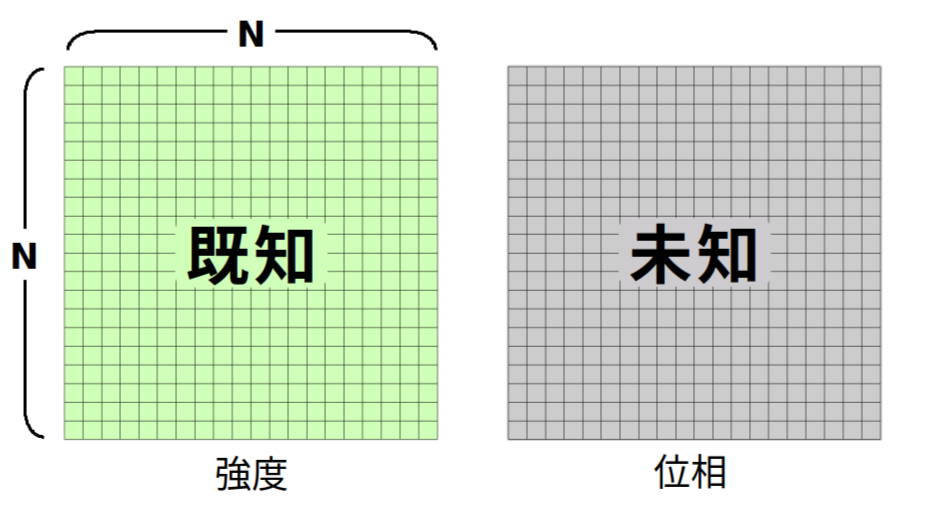
\includegraphics[width=11cm]{phase_retrieval_problem.png}
\caption{位相回復問題}
\label{fig:phase_retrieval_problem}
\end{figure}

\begin{figure}[!ht]
\centering
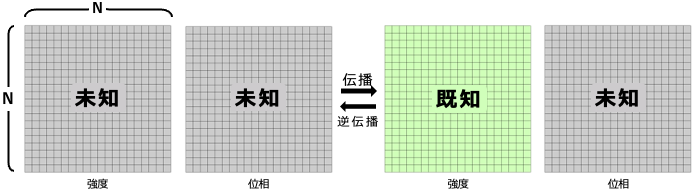
\includegraphics[width=13cm]{phase_retrieval_policy.png}
\caption{位相回復法の方針}
\label{fig:phase_retrieval_policy}
\end{figure}

以下では、代表的な解法を紹介し、続いてそれらを用いた天文用Wolterミラーの波面に対する位相回復法の検討・シミュレーションを行う。

\clearpage
% ================================================== %
% section
% ================================================== %
\newpage

\section{ダイナミックレンジ}
位相回復計算を行う上で非常に重要になるのが、カメラのダイナミックレンジである。
カメラには検出可能な強度範囲と分解能があり、検出したい波面の最大強度が範囲に収まるように取らなければならない。
最大強度が検出可能な範囲に収まるようにNDフィルターなどで光源強度を調節すると、それに応じて検出可能な最小強度が決定される。
例えば、16bitで検出可能なカメラであれば、最大強度の$\frac{1}{65535}$が検出可能な最小強度となり、これより弱い光は強度0として検出される。
このような規格化・量子化を行ったうえで回復できるかどうかを検討することが、位相回復計算の実用において不可欠である。
本研究では、Bitran社のBQ-85Mを用いて計測実験を行う。
そのパラメータを表\ref{tb:ccd_camera_params}に示す。
本章では、ダイナミックレンジを考慮しない理想の系で測定した場合、および示したカメラのダイナミックレンジにおいて測定が可能かどうかを判別する。

\begin{table}[!ht]
\begin{center}
  \begin{tabular}{|c|c|l|} \hline
    項目 & 値 \\ \hline
    製品名 & BQ-85M \\
    ピクセルサイズ & 9.0 um \\
    画素 & 4096 $\times$ 4096 \\
    受光面積 & 36.8 mm $\times$ 36.8 mm \\
    A/Dコンバータ & 16bit (65535階調) \\ \hline
  \end{tabular}
  \caption{CCDカメラのパラメータ}
  \label{tb:ccd_camera_params}
\end{center}
\end{table}

\clearpage
% ================================================== %
% section
% ================================================== %
\newpage

\section{疎条件の利用}
主にCDI(コヒーレント回折イメージング)の文脈において、波動場が到達しない領域を定数0として与えることで、未知数をの総数を激減させるという方法が多く取られる。
CDIとは、図\ref{fig:cdi_schematic}に示すように、サンプルに集光ビームを照射し、その回折像を見ることでそのサンプルの内部構造を解析する方法である。

\begin{figure}[!ht]
\centering
\includegraphics[width=12cm]{cdi_schematic.png}
\caption{コヒーレント回折イメージングの概要}
\label{fig:cdi_schematic}
\end{figure}

位相回復法によってディテクターでの位相およびサンプル面における位相・強度を求めることで、サンプル各点における透過率を求めることが目標となる。
このような系においては、カメラの画素をより細かく取ることにより、対応するサンプル面での領域がサンプルより大きく広がるため、この領域には波面が存在しないという仮定を用いて回復計算を行うことができる。
本研究で対象とするWolterミラーについても、回復の対象である輪帯状でかつ細い波面の面積が下流端開口面全体に対して非常に小さく、同様の方法が有効である可能性がある。
この方針に則って、位相回復計算を行う。
その最もシンプルなアルゴリズムがBIO()である。
疑似コードをAlgorithm\ref{alg:bio}に示す。

\newcommand{\pos} {
    \mathbf{r}
}
\newcommand{\rpos} {
    \mathbf{q}
}

\begin{algorithm}                      
\caption{BIO Algorithm}         
\label{alg:bio}                          
\begin{algorithmic}
    \STATE $\phi_0(\pos)$
      = $\begin{cases}
        \mathrm{rand} & (\pos \in S) \\
        0 & (\pos \notin S)
      \end{cases}$
    \FOR{n = 0 \ldots N-1}
    \STATE $\Psi_n(\rpos) = \mathcal F [\phi_n(\pos)]$
    \STATE $\Psi_{n+1}(\rpos) = \sqrt{I(\rpos)} \exp \left( i \arg \Psi_n(\rpos) \right)$ 
    \STATE $\phi_n'(\pos) = \mathcal F^{-1} [\Psi_{n+1}(\rpos)]$
    \STATE $\phi_{n+1}(\pos)
      = \begin{cases}
          \phi_n'(\pos) & (\pos \in S) \\
          0 & (\pos \notin S)
      \end{cases}$
    \ENDFOR
\end{algorithmic}
\end{algorithm}

これに対して、ほげほげなのがHIO()アルゴリズムである。
疑似コードはAlgorithm\ref{alg:hio}のようになる。

\begin{algorithm}                      
\caption{HIO Algorithm}         
\label{alg:hio}                          
\begin{algorithmic}
    \STATE $\phi_0(\pos)$
      = $\begin{cases}
        \mathrm{rand}(0,1) & (\pos \in S) \\
        0 & (\pos \notin S)
      \end{cases}$
    \FOR{n = 0 \ldots N-1}
    \STATE $\Psi_n(\rpos) = \mathcal F [\phi_n(\pos)]$
    \STATE $\Psi_{n+1}(\rpos) = \sqrt{I(\rpos)} \exp \left( i \arg \Psi_n(\rpos) \right)$ 
    \STATE $\phi_n'(\pos) = \mathcal F^{-1} [\Psi_{n+1}(\rpos)]$
    \STATE $\phi_{n+1}(\pos)
      = \begin{cases}
          \phi_n'(\pos) & (\pos \in S) \\
          \phi_n(\pos) - \beta \phi_n'(\pos) & (\pos \notin S)
      \end{cases}$
    \ENDFOR
\end{algorithmic}
\end{algorithm}

\clearpage
% ================================================== %
% section
% ================================================== %
\newpage

\section{タイコグラフィ法}
\subsection{タイコグラフィ法の概要}
用いるオブジェクトには大きく分けて2種類ある。
1つは透過関数として表現される

\subsection{PIE}
位相回復法は元来、X線顕微鏡として利用されたため、回復の対象はサンプル(オブジェクト)であった。
その最も簡単なタイコグラフィのアルゴリズムがPIE(Ptychography Iterative Engine)である。
これは、照明関数は既知であるとして与え、オブジェクトのみ回復計算を行うアルゴリズムである。
PIEの疑似コードをAlgorighm\ref{alg:pie}に示す。

\begin{algorithm}                      
\caption{PIE Algorithm}         
\label{alg:pie}                          
\begin{algorithmic}
    \STATE $O_0(\pos) = \mathrm{rand}(0,1) \exp(i \mathrm{rand}(0,1) )$
    \FOR{n = 0 \ldots N-1}
      \FOR{j = 0 \ldots M-1}
        \STATE $\psi(\pos_j) = P(\pos) O_n(\pos_j + \pos)$
        \STATE $\Psi(\rpos) = \mathcal F [\psi(\pos)]$
        \STATE $\Psi'(\rpos) = \sqrt{I_j(\rpos)} \exp\left( i \arg \psi(\pos) \right)$ 
        \STATE $\psi'(\pos) = \mathcal F^{-1} [\Psi'(\rpos)]$
        \STATE $O_{n+1}(\pos + \pos_j)'
          = O_n(\pos + \pos_j) 
          + \frac{P_n^*(\pos)}{|P(\pos)|^2+\varepsilon} \left( \psi_n'(\pos) - \psi_n(\pos) \right)$
      \ENDFOR
    \ENDFOR
\end{algorithmic}
\end{algorithm}

逆空間で拘束を掛け、実空間に戻したあとで、オブジェクトを更新する。
オブジェクトの更新則としてシンプルなのは$\psi(\pos_j) = P(\pos) O_n(\pos_j + \pos)$としたのに対応させて$O_{n+1}(\pos_j + \pos) = \frac{\psi'(\pos_j)}{P(\pos)}$とする方法である。
しかし、これは除算に際して発散が起こる可能性があり、実用上大きな問題を孕んでいる。
これを、式\ref{eqn:object_update_derivation}のように変形する。
\begin{eqnarray}
O_{n+1}(\pos_j + \pos)
  &= \frac{\psi'(\pos_j)}{P(\pos)} \nonumber \\
  &= \left( O_n(\pos_j + \pos) - \frac{\psi(\pos_j)}{P(\pos)} \right) + \frac{\psi'(\pos_j)}{P_n(\pos)} \nonumber \\
  &= O_n(\pos_j + \pos) + \frac{1}{P(\pos)} \left( \psi'(\pos_j) - \psi(\pos_j) \right) \label{eqn:object_update_derivation}
\end{eqnarray}

これを一般化して文字を置き換えると、式\ref{eqn:object_update_simplified}のように書ける。
\begin{equation}
\label{eqn:object_update_simplified}
  O_{n+1}(\pos_j + \pos) = O_n(\pos_j + \pos) + w \Delta\psi(\pos)
\end{equation}
この更新の重み$w$を変えることで、アルゴリズムの改善を図る。
発散を回避するため、重みの分母を実数化して微小な定数$\varepsilon$を足して式\ref{eqn:pie_object_update_weight}のように重みを定めたのがAlgorithm\ref{alg:pie}に示したPIEのアルゴリズムである。
\begin{equation}
  \label{eqn:pie_object_update_weight}
  w = \frac{P*(\pos)}{\left| P(\pos) \right|^2 + \varepsilon}
\end{equation}

\subsection{rPIE}
PIEがオブジェクトのみ回復を行っていたのに対して、照明関数も未知として回復計算を行うのがePIE(exteded PIE)である。
ePIEでは式\ref{eqn:pie_object_update_weight}のように定数で発散を回避するのではなく、式\ref{eqn:epie_object_update_weight}のように絶対値の2乗の最大値を取る。
また、更新係数にハイパーパラメタ$\alpha$を掛けることで収束性を上げることができることが知られている。
\begin{equation}
  \label{eqn:epie_object_update_weight}
  w = \alpha \frac{P_n*(\pos)}{\max \left| P_n(\pos) \right|^2}
\end{equation}
ePIEでは照明関数も更新しなければいけないが、これはオブジェクトの更新と同様に式\ref{eqn:epie_probe_update}のように行われる。
\begin{equation}
\label{eqn:epie_probe_update}
  P_{n+1}(\pos) 
  = P_n(\pos) 
  + \beta \frac{O_n*(\pos_j + \pos)}{\max \left| O_n(\pos_j + \pos) \right|^2} \Delta\psi(\pos)
\end{equation}

ePIE(式\ref{eqn:epie_object_update_weight})のように最大値を取る方法に対して、各点での絶対値の2乗とその最大値で重み付き平均を取って分母とするのがrPIE(regularized PIE)である。
更新式は式\ref{eqn:rpie_object_update}および式\ref{eqn:rpie_probe_update}に示す通りである。
rPIEはほとんどePIEの一般化になっている。
\begin{eqnarray}
  O_{n+1}(\pos_j + \pos) &= O_n(\pos_j + \pos) 
    + \frac{P_n*(\pos_j + \pos)}
      {\alpha \max \left| P_n(\pos) \right|^2 + (1-\alpha) \left| P_n(\pos) \right|^2}
    \Delta\psi(\pos) \label{eqn:rpie_object_update} \\
  P_{n+1}(\pos) &= P_n(\pos) 
    + \frac{O_n*(\pos_j + \pos)}
      {\beta \max \left| O_n(\pos_j + \pos) \right|^2 + (1-\beta) \left| O_n(\pos_j + \pos) \right|^2}
    \Delta\psi(\pos) \label{eqn:rpie_probe_update}
\end{eqnarray}

rPIEのアルゴリズムをAlgorithm\ref{alg:rpie}に示す。

\begin{algorithm}                      
\caption{rPIE Algorithm}         
\label{alg:rpie}                          
\begin{algorithmic}
    \STATE $O_0(\pos) = \mathrm{rand}(0,1) \exp(i \mathrm{rand}(0,1) )$
    \STATE $P_0(\pos) = \mathrm{rand}(0,1) \exp(i \mathrm{rand}(0,1) )$
    \FOR{n = 0 \ldots N-1}
      \FOR{j = 0 \ldots M-1}
        \STATE $\psi(\pos_j) = P_n(\pos) O(\pos_j + \pos)$
        \STATE $\Psi(\rpos) = \mathcal F [\psi(\pos)]$
        \STATE $\Psi'(\rpos) = \sqrt{I_j(\rpos)} \exp\left( i \arg \psi(\pos) \right)$ 
        \STATE $\psi'(\pos) = \mathcal F^{-1} [\Psi'(\rpos)]$
        \STATE $O_{n+1}(\pos_j + \pos) 
          = O_n(\pos_j + \pos) + \frac{P_n*(\pos_j + \pos)}
          {\alpha \max \left| P_n(\pos) \right|^2 + (1-\alpha) \left| P_n(\pos) \right|^2}
          \Delta\psi(\pos)$
        \STATE $P_{n+1}(\pos)
          = P_n(\pos) + \frac{O_n*(\pos_j + \pos)}
          {\beta \max \left| O_n(\pos_j + \pos) \right|^2 + (1-\beta) \left| O_n(\pos_j + \pos) \right|^2}
          \Delta\psi(\pos)$
      \ENDFOR
    \ENDFOR
\end{algorithmic}
\end{algorithm}

\clearpage
% ================================================== %
% section
% ================================================== %
\newpage

\section{ディテクター走査による冗長性}


\clearpage
% ================================================== %
% section
% ================================================== %
\newpage

\section{下流端開口走査による冗長性}

\subsection{対称性}

\clearpage
% ================================================== %
% section
% ================================================== %
\newpage


\section{結論}
\label{chap3_conclusion}
結論を述べる。




%%%%%%%%%%%%%%%%%%%%%%%%%%%%%%%%%%%%%%%%%%%%%%%%%%%%%%%%%%%%%%%%%%%%%%%%%%%%%
%%% Local Variables:
%%% mode: katex
%%% TeX-master: "../thesis"
%%% End:
